\documentclass[a4paper,12pt]{article} % This defines the style of your paper

\usepackage[top = 2.5cm, bottom = 2.5cm, left = 2.5cm, right = 2.5cm]{geometry} 

% Unfortunately, LaTeX has a hard time interpreting German Umlaute. The following two lines and packages should help. If it doesn't work for you please let me know.
\usepackage[T1]{fontenc}
\usepackage[utf8]{inputenc}
\usepackage{subcaption}

% The following two packages - multirow and booktabs - are needed to create nice looking tables.
\usepackage{multirow} % Multirow is for tables with multiple rows within one cell.
\usepackage{booktabs} % For even nicer tables.
\usepackage{amsmath}
\usepackage{bm}

% As we usually want to include some plots (.pdf files) we need a package for that.
\usepackage{graphicx} 
\usepackage{rotating}
\usepackage{cancel}

% The default setting of LaTeX is to indent new paragraphs. This is useful for articles. But not really nice for homework problem sets. The following command sets the indent to 0.
\usepackage{setspace}
\setlength{\parindent}{0in}

% Package to place figures where you want them.
\usepackage{float}

% The fancyhdr package let's us create nice headers.
\usepackage{fancyhdr}

\usepackage[utf8]{inputenc}
\usepackage[portuguese]{babel}
\usepackage{makecell}
\usepackage{listings}
\usepackage{xcolor}
\usepackage[colorlinks=true]{hyperref}


\hypersetup{
    allcolors=blue,
}
\definecolor{codegreen}{rgb}{0,0.6,0}
\definecolor{codegray}{rgb}{0.5,0.5,0.5}
\definecolor{codepurple}{rgb}{0.58,0,0.82}
\definecolor{backcolour}{rgb}{0.95,0.95,0.92}

\lstdefinestyle{mystyle}{
    backgroundcolor=\color{backcolour},   
    commentstyle=\color{codegreen},
    keywordstyle=\color{magenta},
    numberstyle=\tiny\color{codegray},
    stringstyle=\color{codepurple},
    basicstyle=\ttfamily\footnotesize,
    breakatwhitespace=false,         
    breaklines=true,                 
    captionpos=b,                    
    keepspaces=true,                 
    numbers=left,                    
    numbersep=5pt,                  
    showspaces=false,                
    showstringspaces=false,
    showtabs=false,                  
    tabsize=2
}
\lstset{style=mystyle}
\renewcommand{\arraystretch}{1.5}

\pagestyle{fancy} % With this command we can customize the header style.

\fancyhf{} % This makes sure we do not have other information in our header or footer.

\lhead{\footnotesize Homework 4}% \lhead puts text in the top left corner. \footnotesize sets our font to a smaller size.

%\rhead works just like \lhead (you can also use \chead)
\rhead{\footnotesize Joana Pimenta, Rodrigo Laia} %<---- Fill in your lastnames.

% Similar commands work for the footer (\lfoot, \cfoot and \rfoot).
% We want to put our page number in the center.
\cfoot{\footnotesize \thepage} 

\begin{document}

\thispagestyle{empty} % This command disables the header on the first page. 

\begin{tabular}{p{15.5cm}} % This is a simple tabular environment to align your text nicely 
{\large \bf Aprendizagem} \\
Instituto Superior Técnico \\ outubro  de 2023  \\ \\ 
\hline % \hline produces horizontal lines.
\\
\end{tabular} % Our tabular environment ends here.

\vspace*{0.3cm} % Now we want to add some vertical space in between the line and our title.

\begin{center} % Everything within the center environment is centered.
	{\Large \bf Homework 4 - Report} % <---- Don't forget to put in the right number
	\vspace{2mm}
	
        % YOUR NAMES GO HERE
	{\bf Joana Pimenta (103730), Rodrigo Laia (102674) } % <---- Fill in your names here!
		
\end{center}  

\vspace{0.4cm}

\section*{Pen and Paper}
\begin{enumerate}

\item Fórmulas utilizadas:

\begin{equation}
    \gamma_{ki} = p(c_k|\mathbf{x}_i) = \frac{p(c_k)p(\mathbf{x}_i|c_k)}{p(\mathbf{x}_i)}
\end{equation}

\begin{equation}
    p(\mathbf{x}_i) = p(c_1)p(\mathbf{x}_i|c_1)+p(c_2)p(\mathbf{x}_i|c_2)
\end{equation}

\begin{equation}
    p(\mathbf{x}_i|c_k) =
    \begin{cases} 
        p_{k} \cdot \mathcal{N}(\mathbf{x}_i|\boldsymbol{\mu}_k,\boldsymbol{\Sigma}_k) & \text{se } y_1 = 1 \\
        (1-p_k) \cdot \mathcal{N}(\mathbf{x}_i|\boldsymbol{\mu}_k,\boldsymbol{\Sigma}_k) & \text{se } y_1 = 0 
    \end{cases}
    \label{eq:p_xi_ck}
\end{equation}

\begin{equation}
    p(c_k) = \pi_k
\end{equation}

\textbf{E-step:} \\

Cálculo das probabilidades $p(\textbf{x}_i)$
\begin{center}
\begin{tabular}{c|c}

$\mathbf{x}_i$ & $p(\mathbf{x}_i)$ \\
\hline
$\mathbf{x}_1$ & 0.05185 \\
$\mathbf{x}_2$ & 0.02775 \\
$\mathbf{x}_3$ & 0.04337 \\
$\mathbf{x}_4$ & 0.05243 \\

\end{tabular}
\end{center}



Cálculos dos $\gamma_{ki}$

\begin{center}
\begin{tabular}{c|c|c}
$i$ & $\gamma_{k=1,i}$ & $\gamma_{k=2,i}$ \\
\hline
1 & 0.19259 & 0.80741 \\
2 & 0.63135 & 0.36865 \\
3 & 0.55181 & 0.44819 \\
4 & 0.16892 & 0.83108 \\
\end{tabular}
\end{center}

\textbf{M-step:} \\ \\
Cada observação $\mathbf{x}_i$ permite atualizar os parâmetros com peso $\gamma_{ki}$. 
Assim calculamos os novos parâmetros atualizados para cada cluster utilizando as seguintes fórmulas. 

\begin{equation}
    N_k = \sum_{i=1}^4 \gamma_{ki}
\end{equation}

\begin{equation}
    \pi_k = \frac{N_k}{N}
\end{equation}
% o parâmetro de uma distribuição de Bernoulli é a probabilidade de sucesso, 
% ou seja, a probabilidade de a y_1 assumir o valor 1.
% Ela é dada pelo numero total de observações em que y_1 é 1 dividido pelo numero total de observações
% no entanto, neste caso cada observação tem um peso diferente, dado pelo gamma_ki
% assim, o parâmetro da distribuição de Bernoulli é dado por:
\begin{equation}
    P_k(y_1=1) = \frac{\sum_{i=1}^4 \gamma_{ki} \cdot p(y_1=1|\mathbf{x}_i)}{\sum_{i=1}^4 \gamma_{ki}} 
\end{equation}
Nota: A probabilidade $p(y_1=1|\mathbf{x}_i)$ é 1 se $y_1$ de $\mathbf{x}_i$ for 1 e 0 caso contrário. 

\begin{equation}
    \boldsymbol{\mu}_k = \frac{1}{N_k} \sum_{i=1}^4 \gamma_{ki} \mathbf{x}_i    
\end{equation}

\begin{equation}
    \boldsymbol{\Sigma}_k = \frac{1}{N_k} \sum_{i=1}^4 \gamma_{ki} (\mathbf{x}_i - \boldsymbol{\mu}_k)(\mathbf{x}_i - \boldsymbol{\mu}_k)^T
\end{equation}


Parâmetros atualizados:

\begin{equation*}
    \pi_1 = 0.38617
\end{equation*}

\begin{equation*}
    \pi_2 = 0.61383
\end{equation*}

\begin{equation*}
    P_{k=1}(y_1=1) = 0.23404
\end{equation*}

\begin{equation*}
    P_{k=2}(y_1=1) = 0.66732
\end{equation*}

\begin{equation*}
    \boldsymbol{\mu}_1 = \begin{bmatrix}
    0.02651 \\
    0.50713
\end{bmatrix}
\end{equation*}

\begin{equation*}
    \boldsymbol{\mu}_2 = \begin{bmatrix}
    0.30914 \\
    0.21042
\end{bmatrix}
\end{equation*}

\begin{equation*}
    \boldsymbol{\Sigma}_1 = \begin{bmatrix}
    0.14137 & -0.10541 \\
    -0.10541 & 0.09605
\end{bmatrix}
\end{equation*}

\begin{equation*}
    \boldsymbol{\Sigma}_2 = \begin{bmatrix}
    0.10829 & -0.08865 \\
    -0.08865 & 0.10412
\end{bmatrix}
\end{equation*}

\item
Para calcular os posteriors da observação $\mathbf{x}_{new}$ utilizamos a 
seguinte fórmula:

\begin{equation}
    p(cluster = k|\mathbf{x}_{new}) = \frac{p(cluster = k)p(\mathbf{x}_{new}|cluster = k)}{p(\mathbf{x}_{new})}
\end{equation}

Em que $p(cluster = k)$ é dado por $\pi_k$ e $p(\mathbf{x}_{new}|cluster = k)$ é dado pela fórmula ~\eqref{eq:p_xi_ck}.

Cálculos:

\begin{equation*}
    p(\mathbf{x}_{new}) = 0.03048
\end{equation*}

\begin{equation*}
    p(cluster = 1|\mathbf{x}_{new}) = 0.08029
\end{equation*}

\begin{equation*}
    p(cluster = 2|\mathbf{x}_{new}) = 0.91971
\end{equation*}

Assim conclui-se que a observação $\mathbf{x}_{new}$ pertence ao cluster 2 com probabilidade 0.91971
e ao cluster 1 com probabilidade 0.08029.

\item Neste exercício assumimos que o cluster atribuído a cada observação é 
é escolhido pelo critério de \textit{maximum likelihood}.
Assim, o cluster escolhido é dado por:

\begin{equation}
    cluster = \arg\max_k p(\mathbf{x}_i|cluster = k)
\end{equation}

Em que $p(\mathbf{x}_i|cluster = k)$ é dado pela fórmula ~\eqref{eq:p_xi_ck}. \\ \\

Assim,

\begin{table}[H]
\centering
\begin{tabular}{|c|c|c|c|}
\hline
Observação & $p(\mathbf{x}_i|cluster = 1)$ & $p(\mathbf{x}_i|cluster = 2)$ & Cluster atribuído\\ \hline
$\mathbf{x_1}$ &  0.23147  & 0.94954 & 2 \\ \hline
$\mathbf{x_2}$ &  1.26633  & 0.08874 & 1 \\ \hline
$\mathbf{x_3}$ &  1.43811  & 0.45417 & 1 \\ \hline
$\mathbf{x_4}$ &  0.02077  & 0.72331 & 2 \\ \hline
\end{tabular}
\end{table}


Coeficiente de Silhueta:

\begin{equation}
    s_i = 1 - \frac{a(\mathbf{x}_i)}{b(\mathbf{x}_i)}
\end{equation}

em que $a(\mathbf{x}_i)$ é a distância média entre $\mathbf{x}_i$ e as outras 
observações no mesmo cluster e $b(\mathbf{x}_i)$ é a distância média entre 
$\mathbf{x}_i$ e as observações no outro cluster. \\ \\

A silhueta de um cluster é dada pela média dos coeficientes de silhueta de todas
as observações pertencentes a esse cluster. \\ \\

A silhueta da solução é por sua vez dada pela média das silhuetas de todos os
clusters. \\ \\

Neste caso a distância considerada é a distância de Manhattan, logo:

\begin{equation}
    d(\mathbf{u},\mathbf{v}) = \sum_{i=1}^n |u_i - v_i|
\end{equation}

Cálculo das distâncias:

\begin{equation*}
    d(\mathbf{x}_1,\mathbf{x}_2) = 2.7
\end{equation*}

\begin{equation*}
    d(\mathbf{x}_1,\mathbf{x}_3) = 1.7(9)
\end{equation*}

\begin{equation*}
    d(\mathbf{x}_1,\mathbf{x}_4) = 0.3(9)
\end{equation*}

\begin{equation*}
    d(\mathbf{x}_2,\mathbf{x}_3) = 1.9
\end{equation*}

\begin{equation*}
    d(\mathbf{x}_2,\mathbf{x}_4) = 2.7
\end{equation*}

\begin{equation*}
    d(\mathbf{x}_3,\mathbf{x}_4) = 1.7(9)
\end{equation*}

Assim, as silhuetas obtidas foram:

\begin{table}[H]
\centering
\begin{tabular}{|c|c|c|c|c|c|c|}
\hline
cluster           & $\mathbf{x}_i$ & a$(\mathbf{x}_i)$ & b$(\mathbf{x}_i)$ & s$(\mathbf{x}_i)$  & s(cluster)& s(sol)\\ \hline
\multirow{2}{*}{1} & $\mathbf{x}_2$ & 0.9 & 2.7 & 0.(6)  & \multirow{2}{*}{0.58(3)} & \multirow{4}{*}{0.702(7)} \\ \cline{2-5}
                    & $\mathbf{x}_3$ & 0.9 & 1.7(9) & 0.4(9) & &  \\ \cline{1-6}
\multirow{2}{*}{2} & $\mathbf{x}_1$ & 0.3(9) & 2.25 &0.8(2) & \multirow{2}{*}{0.8(2)}  & \\ \cline{2-5}
                    & $\mathbf{x}_4$ & 0.3(9) & 2.25 & 0.8(2) &  &   \\ \hline
\end{tabular}
\end{table}

\item

A purity é dada por:

\begin{equation}
    \text{purity} = \frac{1}{N} \sum_{k=1}^K \max_j |c_k \cap t_j| = \frac{1}{N} \left( \max_j |c_1 \cap t_j| + \max_j |c_2 \cap t_j| \right)
\end{equation}


Uma vez que temos uma purity de 0.75 e um número total de observações de 4,
então $\left( \max_j |c_1 \cap t_j| + \max_j |c_2 \cap t_j| \right) = 0.75 \times 4 = 3$ \\ 

Logo podemos ter os seguintes casos:
\begin{enumerate}
    \item $\max_j |c_1 \cap t_j| = 3$ e $\max_j |c_2 \cap t_j| = 0$
    \item $\max_j |c_1 \cap t_j| = 2$ e $\max_j |c_2 \cap t_j| = 1$
    \item $\max_j |c_1 \cap t_j| = 1$ e $\max_j |c_2 \cap t_j| = 2$
    \item $\max_j |c_1 \cap t_j| = 0$ e $\max_j |c_2 \cap t_j| = 3$
\end{enumerate}

As opções (a) e (d) não são possíveis porque os clusters 2 e 1 só têm 2 observações cada um. 

\textbf{Opção (b)} \\ 
Neste caso, as observações do cluster 1 são as duas classificadas corretamente. 
No cluster 2 uma é corretamente identificada e a outra não. Assim, as observações 
no cluster 1 têm a mesma classificação; uma das observações do cluster 2 tem classificação
diferente das do cluster 1 e a outra pode ter classificação igual às do cluster 1 (opção 1)
ou diferente, sendo que neste caso é também diferente da classificação do outra observação
do cluster 2 (opção 2). Assim, conclui-se que o número verdadeiro de classes pode ser 2 ou 3. \\
Para visualizar melhor as opções possíveis fizemos os seguintes esquemas 
(bolas de cores diferentes representam classes verdadeiras diferentes):

\begin{figure}[H]
\centering
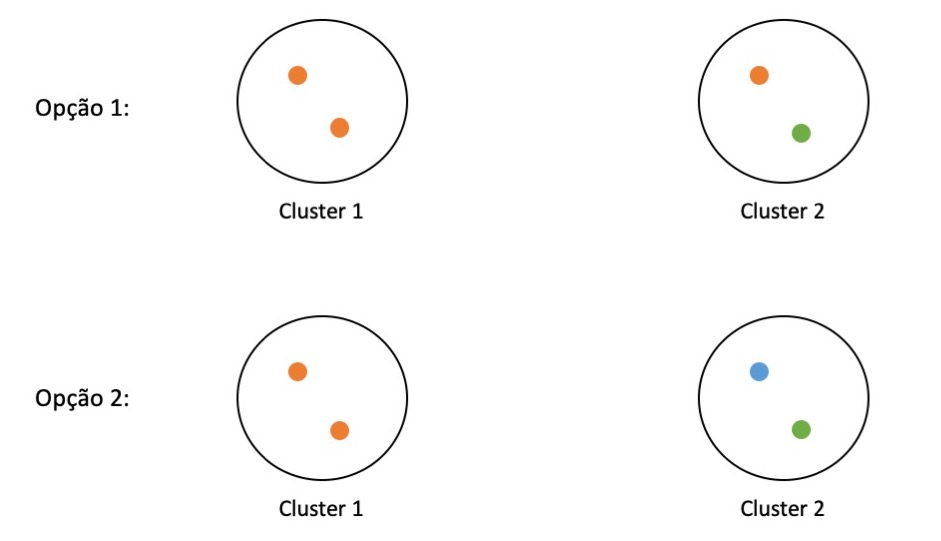
\includegraphics[width=0.7\textwidth]{ex4_clusters.jpg}
\end{figure}

\textbf{Opção (c)} \\
O raciocínio é semelhante ao da opção (b). Conclui-se que o número verdadeiro de classes pode ser 2 ou 3.

\end{enumerate}

\clearpage

\section*{Programming - Código Python e Resultados Obtidos}

\begin{enumerate}

\item 

Usando o sklearn, aplicámos clustering K-means totalmente não supervisionada nos dados normalizados com valores de k $\in$ {2, 3, 4, 5} (usando random state=0). Calculámos a silhueta e a pureza para cada valor de k. \\ \\

Os gráficos obtidos foram os seguintes:

\begin{figure}[H]
    \begin{minipage}{.5\textwidth}
      \centering
      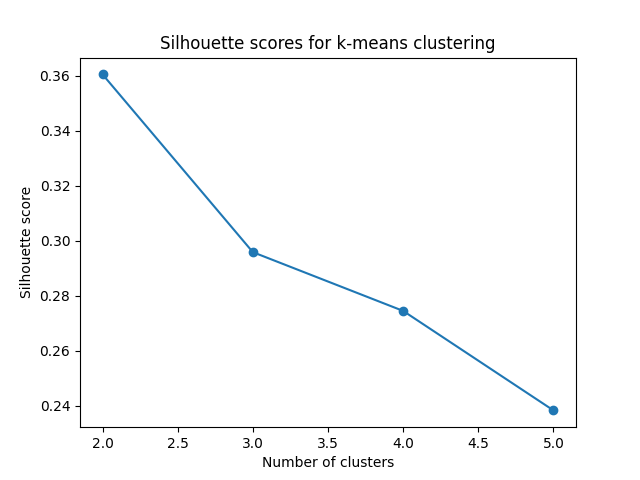
\includegraphics[width=\linewidth]{ex1_silhouette.png}
      \captionsetup{font=small} 
      \caption{Valores de silhueta para diferentes  k}
    \end{minipage}%
    \begin{minipage}{.5\textwidth}
      \centering
      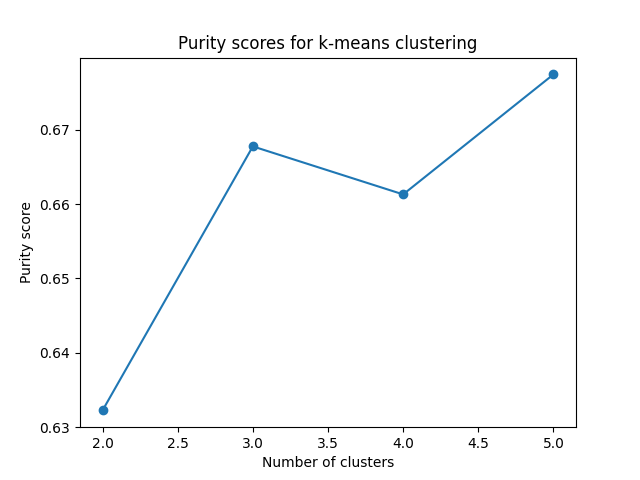
\includegraphics[width=\linewidth]{ex1_purity.png}
      \captionsetup{font=small} 
      \caption{Valores de pureza para diferentes k}
    \end{minipage}
    \end{figure}

Foi possível observar que, de um modo geral, a pureza aumenta com o número de clusters, enquanto que a silhueta diminui. 
Ou seja, com o aumento do k, os clusters ficam pior definidos (menos coesos e mais juntos porque a silhueta diminui) mas também mais homogéneos (pureza aumenta). \\

Código Utilizado:

\begin{lstlisting}[language=Python]
def purity_score(y_true, y_pred):
    # compute contingency/confusion matrix
    confusion_matrix = metrics.cluster.contingency_matrix(y_true, y_pred)
    return np.sum(np.amax(confusion_matrix, axis=0)) / np.sum(confusion_matrix) 

silhouettes = []
purities = []
for k in range(2, 6):
    kmeans_algo = cluster.KMeans(n_clusters=k, random_state=0)
    kmeans_model = kmeans_algo.fit(features_scaled)
    target_pred = kmeans_model.labels_
    purity = purity_score(target, target_pred)
    silhouette = metrics.silhouette_score(features_scaled, target_pred)
    silhouettes.append(silhouette)
    purities.append(purity)
    
    print("Purity score for k = " , str(k) , " is " , purity)
    print("Silhouette score for k = " , str(k) , " is " , silhouette)
    
#Plot Silhouette
plt.plot([2,3,4,5], silhouettes, 'o-')
plt.title('Silhouette scores for k-means clustering')
plt.xlabel('Number of clusters')
plt.ylabel('Silhouette score')
plt.savefig('ex1_silhouette.png')
plt.show()

#Plot Purity
plt.plot([2,3,4,5], purities, 'o-')
plt.title('Purity scores for k-means clustering')
plt.xlabel('Number of clusters')
plt.ylabel('Purity score')
plt.savefig('ex1_purity.png')
plt.show()
\end{lstlisting}

\item

Considerando a aplicação do PCA depois da normalização dos dados, identificámos a variabilidade explicada 
pelos dois primeiros componentes principais.\\

Concluímos que as componentes principais (eigenvectors) são:
\begin{itemize}
    \item PC1: (0.59162, 0.46704, 0.51508, 0.32569, -0.11582, 0.21693)
    \item PC2: (0.10004, -0.67037, 0.08005, 0.44333, -0.58107, 0.00458)
\end{itemize}
Obtivemos os seguintes valores para a variabilidade explicada:\\
Explained variance (ratio) = (0.56181, 0.20956)\\

Somando as duas variabilidades explicadas, obtemos 0.77137, ou seja, 77.137\% da variabilidade é explicada pelas duas componentes principais. Neste caso, uma variabilidade considerável é explicada com apenas duas componentes principais.
O PCA é bastante útil porque permite reduzir as dimensões do dataset utilizando a informação mais relevante para estudar o mesmo.   \\

Para cada uma das duas componentes principais, ordenámos as variáveis de entrada por relevância. \\

Concluímos que as variáveis mais importantes para a primeira componente principal são: 
\begin{itemize}
    \item pelvic incidence :  0.44394
    \item lumbar lordosis angle :  0.38651
    \item pelvic tilt :  0.35046
    \item sacral slope :  0.24439
    \item degree spondylolisthesis :  0.16278
    \item pelvic radius :  0.08691
\end{itemize}

As variáveis mais importantes para a segunda componente principal são: 
\begin{itemize}
    \item pelvic tilt :  0.37797
    \item pelvic radius :  0.32762
    \item sacral slope :  0.24994
    \item pelvic incidence :  0.05640
    \item lumbar lordosis angle :  0.04513
    \item degree spondylolisthesis :  0.00258
\end{itemize}

Por fim, ordenámos as variáveis por relevância para as duas componentes principais: 
\begin{itemize}    
    \item pelvic tilt :  0.51544
    \item pelvic incidence :  0.44751
    \item lumbar lordosis angle :  0.38913
    \item sacral slope :  0.34957
    \item pelvic radius :  0.33895
    \item degree spondylolisthesis :  0.16280 \\
\end{itemize} 

Entender a importância de cada variável nas componentes principais é crucial para interpretar e 
utilizar de forma eficiente a técnica do PCA e ajuda a melhorar a qualidade das análises. \\

Código Utilizado:

\begin{lstlisting}[language=Python]
pca = PCA(n_components=2)
pca.fit(features_scaled)
X_pca = pca.transform(features_scaled)

print("Components (eigenvectors):\n",pca.components_)
print("Explained variance (ratio) =",pca.explained_variance_ratio_)

xvector = pca.components_[0] * max(X_pca[:,0])
yvector = pca.components_[1] * max(X_pca[:,1])

columns = features.columns
features1_rel = {columns[i] : math.sqrt(xvector[i]**2) for i in range(len(columns))}
sorted_features1 = sorted(zip(features1_rel.values(), features1_rel.keys()),reverse=True)
print('Features sorted by relevance for the first component: \n')
for i in range(len(sorted_features1)):
    print(f'{sorted_features1[i][1]} : {sorted_features1[i][0]: .5f}')

features2_rel = {columns[i] : math.sqrt(yvector[i]**2) for i in range(len(columns))}
sorted_features2 = sorted(zip(features2_rel.values(), features2_rel.keys()),reverse=True)
print('\nFeatures sorted by relevance for the second component: \n')
for i in range(len(sorted_features2)):
    print(f'{sorted_features2[i][1]} : {sorted_features2[i][0]: .5f}')

features_rel = {columns[i] : math.sqrt(xvector[i]**2 + yvector[i]**2) for i in range(len(columns))}
sorted_features = sorted(zip(features_rel.values(), features_rel.keys()),reverse=True)
print('\nFeatures sorted by relevance: \n')
for i in range(len(sorted_features)):
    print(f'{sorted_features[i][1]} : {sorted_features[i][0]: .5f}')
    
\end{lstlisting}

\item Visualizar os dados com ground diagnosis e os clusters obtidos para k = 3 projetando os dados normalizados num espaço bidimensional PCA. \\

\begin{figure}[H]
      \centering
      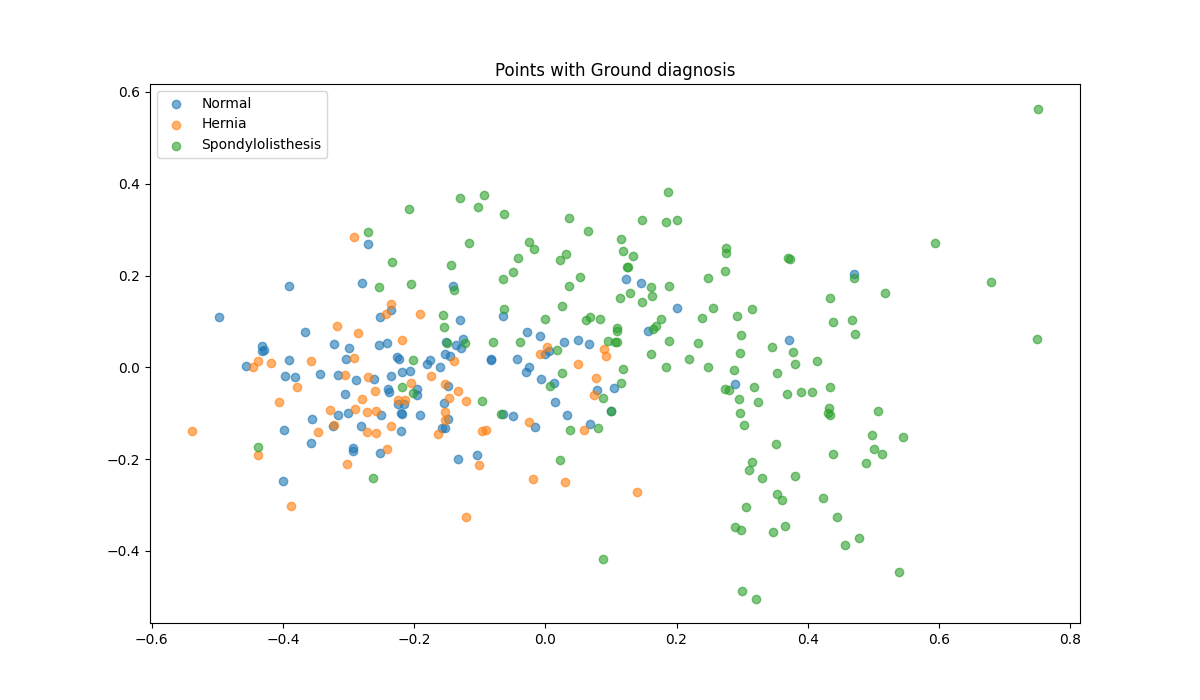
\includegraphics[width=0.8\linewidth]{ex3_ground_diagnosis.png}
      \captionsetup{font=small} 
      \caption{Pontos com Ground Diagnosis}
\end{figure}

\begin{figure}[H]
    \centering
    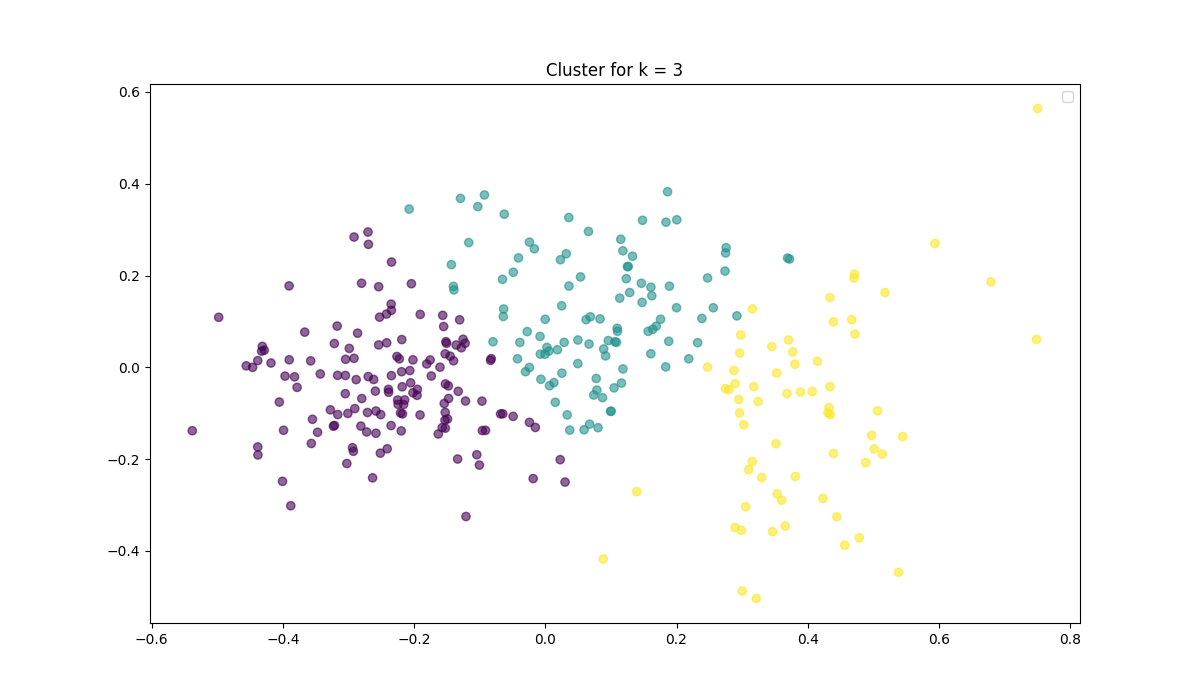
\includegraphics[width=0.8\linewidth]{ex3_cluster.png}
    \captionsetup{font=small} 
    \caption{Clusters para k = 3}
\end{figure}

\begin{figure}[H]
    \centering
    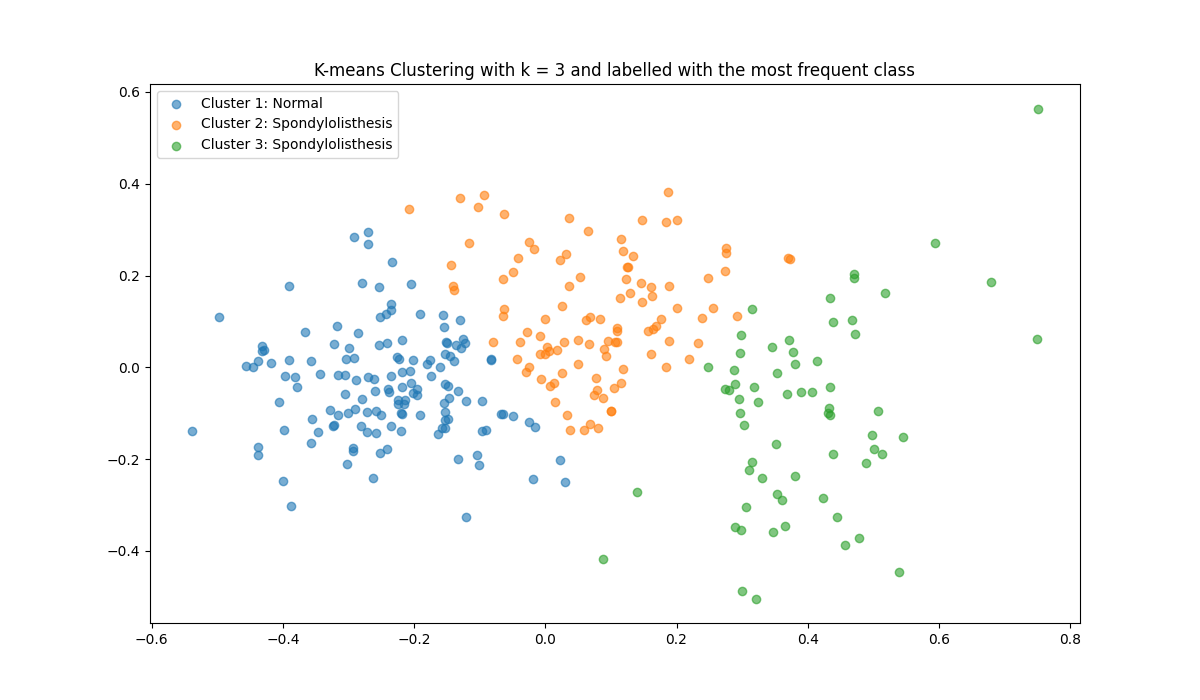
\includegraphics[width=0.8\linewidth]{ex3_cluster_labelled.png}
    \captionsetup{font=small} 
    \caption{Clusters para k = 3 com a classe mais frequente}
\end{figure}

No segundo gráfico, visualizamos os pontos separados em 3 clusters. Tendo em conta o primeiro e segundo gráficos, é possível observar que o algoritmo de clustering não conseguiu separar os pontos de forma a que cada cluster correspondesse a uma classe, notando que o cluster menos heterogéneo é o roxo (segundo gráfico). \\
No ultimo gráfico desta secção, visualizamos os pontos separados em 3 clusters e com a classe mais frequente em cada cluster. \\

Código Utilizado: 

\begin{lstlisting}[language=Python]
# i)
plt.figure(figsize=(12,7))
plt.scatter(X_pca[target=='Normal', 0], X_pca[target=='Normal', 1], alpha=0.6, label='Normal')
plt.scatter(X_pca[target=='Hernia', 0], X_pca[target=='Hernia', 1], alpha=0.6, label='Hernia')
plt.scatter(X_pca[target=='Spondylolisthesis', 0], X_pca[target=='Spondylolisthesis', 1], alpha=0.6, label='Spondylolisthesis')

plt.legend()
plt.title('Points with Ground diagnosis')
plt.savefig('ex3_ground_diagnosis.png')
plt.show()

# ii)

kmeans_algo = cluster.KMeans(n_clusters=3, random_state=0)
kmeans_model = kmeans_algo.fit(features_scaled)
target_pred = kmeans_model.labels_

plt.figure(figsize=(12, 7))
plt.scatter(X_pca[:,0], X_pca[:,1], c=target_pred, alpha=0.6)

plt.legend()
plt.title('Cluster for k = 3')
plt.savefig('ex3_cluster.png')
plt.show()

# iii)

cluster_mapping = pd.DataFrame({'Cluster': target_pred, 'Class': target})

# Calculate the mode class for each cluster
cluster_mode = cluster_mapping.groupby('Cluster')['Class'].agg(lambda x: x.mode().iat[0])

plt.figure(figsize=(12, 7))
for cluster in set(target_pred):
    data = X_pca[target_pred == cluster]
    plt.scatter(data[:, 0], data[:, 1], label=f'Cluster {cluster}', alpha=0.6)

plt.title('K-means Clustering with k = 3 and labelled with the most frequent class') 
plt.savefig('ex3_cluster_labelled.png')
# Create a legend using the calculated mode class for each cluster
legend_labels = [f'Cluster {cluster+1}: {mode_class}' for cluster, mode_class in cluster_mode.items()]
plt.legend(legend_labels)

# Show the plot
plt.show()
\end{lstlisting}

\item 

Com base nos resultados obtidos nas questões anteriores, concluímos que é possível utilizar o clustering para realizar diagnósticos, identificando grupos de pacientes com características semelhantes, ou decidir qual o melhor tipo de tratamento 
consoante as diferentes características entre os indivíduos da população identificada com uma doença. Através desses subgrupos de indivíduos com características semelhantes é possível identificar outros tipos da doença.

Também se usa esta técnica para criar perfis de risco com base nas características da população. Isso pode ser usado para implantar programas de combate a aos riscos específicos da mesma.

Analisar mais profundamente os dados de cada cluster poderá a ajudar os profissionais a compreender melhor a natureza do problema, diferentes formas de como o diagnosticar e, posteriormente, tratar.

Contudo, a utilização do clustering requer bastante cuidado visto que é preciso equilibrar os valores de silhueta e de pureza (consoante a informação que pretendemos retirar dos dados) e dado que os clusters nem sempre representam indivíduos exclusivamente da mesma classe. Neste caso, os plots anteriores revelaram a dificuldade do algoritmo em separar as populações das pessoas com classe Hérnia e Normal.

\end{enumerate}

\end{document}
